\section{\acs{1D} Datasets}

In order to assess the estimation routine proposed in Chapter \ref{chap:theory}
-- specifically the effectiveness of applying \ac{NLP} using an initial guess
generated using the \ac{MPM} -- a series of synthetic \acp{FID} were constructed
using \eqref{eq:hypercomplex-fid}. For each \ac{FID}, a model order of $M=20$
was used, the number of points sampled was $\None = 1024$, the sweep width
was $\fswone=\qty{125}{\hertz}$, and the transmitter offset was $\foffone =
\qty{0}{\hertz}$.  Each oscillator was assigned a phase of \ang{0}, while the
amplitudes, frequencies and damping factors were drawn at random from the
following distributions:
$\bdam \sim \mathcal{U}(1, 5)$, $\bdfonem \sim \mathcal{U}(\qty{-55}{\hertz},
\qty{55}{\hertz})$, $\bdetaonem \sim \mathcal{U}(\qty{2}{\per\second},
\qty{8}{\per\second})\ \forall m \in \lbrace 0, \cdots, 19\rbrace$. An extra
constraint was applied to the frequencies,
such that no two oscillators were permitted to have frequencies that differed
by less than $\nicefrac{4 \fswone}{\None} \approx \qty{0.49}{\hertz}$. Each
noiseless \ac{FID} was then corrupted with \ac{AWGN}, with a target \ac{SNR} of
\qty{25}{\deci\bel}\note{Reference that this is the lowest
SNR that the MPM considered to be effective}. The spectra of the simulated
\acp{FID} are presented in panel a of Figure \ref{fig:mpm_vs_nlp}.

For each \ac{FID}, the \ac{MPM} was performed, assuming that the model order is
30, constituting a considerable over-fit. Simulated signals typically show a
clean division between signal and noise components, with noise components
commonly being characterised by small amplitudes and/or very small damping
factors. For this reason, prior to subjecting the \ac{MPM} result to \ac{NLP},
oscillators which satisfied either $\bdam < 0.1$ or  $\bdetaonem <
\qty{0.7}{\per\second}$ were removed from the parameter set. The individual
oscillators which make up the \ac{MPM} result after purging are displayed in panel b of
Figure \ref{fig:mpm_vs_nlp}, along with the residual between the data and the
model.

It can be seen that in several spectral regions across the datasets, especially
those which are more crowded, oscillators possess parameters which deviate
significantly from the true parameters (the true set of oscillators is
presented in panel d), with the most notable feature being individual
oscillator phases, which can stray far from \ang{0}.
The central motivation behind employing phase variance-regularised \ac{NLP} is
as a means of attempting to overcome this detrimental feature of the \ac{MPM}.
It should be noted however, that the \ac{MPM} invariably generates a model with
good agreement with the data, as evidenced by the residual.
In Figure \ref{fig:mpm_vs_nlp}, the blue oscillators are those which agree very
closely with a particular oscillator in the true set of parameters. Oscillators
with other colours are in disagreement for some reason (\textit{vide infra}).
The goal of the \ac{NLP} routine is therefore to adjust the parameters
describing the non-blue oscillators in panel b such that they agree with
oscillators found in the true set, while not affecting the blue oscillators.
The results of \ac{NLP} at convergence ($\epsilon = \num{1e-8}$) are provided
in panel c. ...

\note{Maybe define the notion of a ``frequency neighbourhood''?
    A small rage of frequencies within which it is necessary for the MPM to generate at least the same number of oscillators as the true number for NLP to have a chance of correctly estimating the dataset.
}

\paragraph{Green oscillators}
These oscillators belong to a grouping of oscillators with similar frequencies
which exhibited significant deviation from the true parameter set, but which
were mapped to agree closely with the true result thanks to the \ac{NLP}
routine.

\paragraph{Orange oscillators}
Orange oscillators are examples of scenarios where the \ac{MPM} routine
over-fit a particular spectral region, and the \ac{NLP} routine was able to
purge these excessive oscillators, leading to a parsimonious set of parameters.

\paragraph{Red oscillators}
These oscillators are examples of a cases where the routine has underfit the
dataset, because there are a pair of similar-frequency oscillators in the true
parameter set which were not be individually resolved. In these cases, the
\ac{MPM} assigned only a single oscillator to fit the spectral region, making
it impossible for the \ac{NLP} routine to make any improvements to the
estimation result.

\paragraph{Yellow oscillators}
Similar to red oscillators, yellow oscillators eventually lead to the
under-fitting of the dataset. However, in these cases, the \ac{MPM} has
generated sufficient oscillators in the frequency neighbourhood. Unlike in
scenarios which is seen for the green oscillators though, the \ac{NLP} routine
evolves such that at least one of the oscillators is driven by the phase
variance constraint to acquire a negative amplitude, such that it is purged
from the parameter set. This typically occurs when an oscillator has an initial
phase close to \ang{180}.

\paragraph{Purple oscillators}
The arise rather infrequently, and correspond to over-fits of the dataset.


\begin{sidewaysfigure}
    \centering
    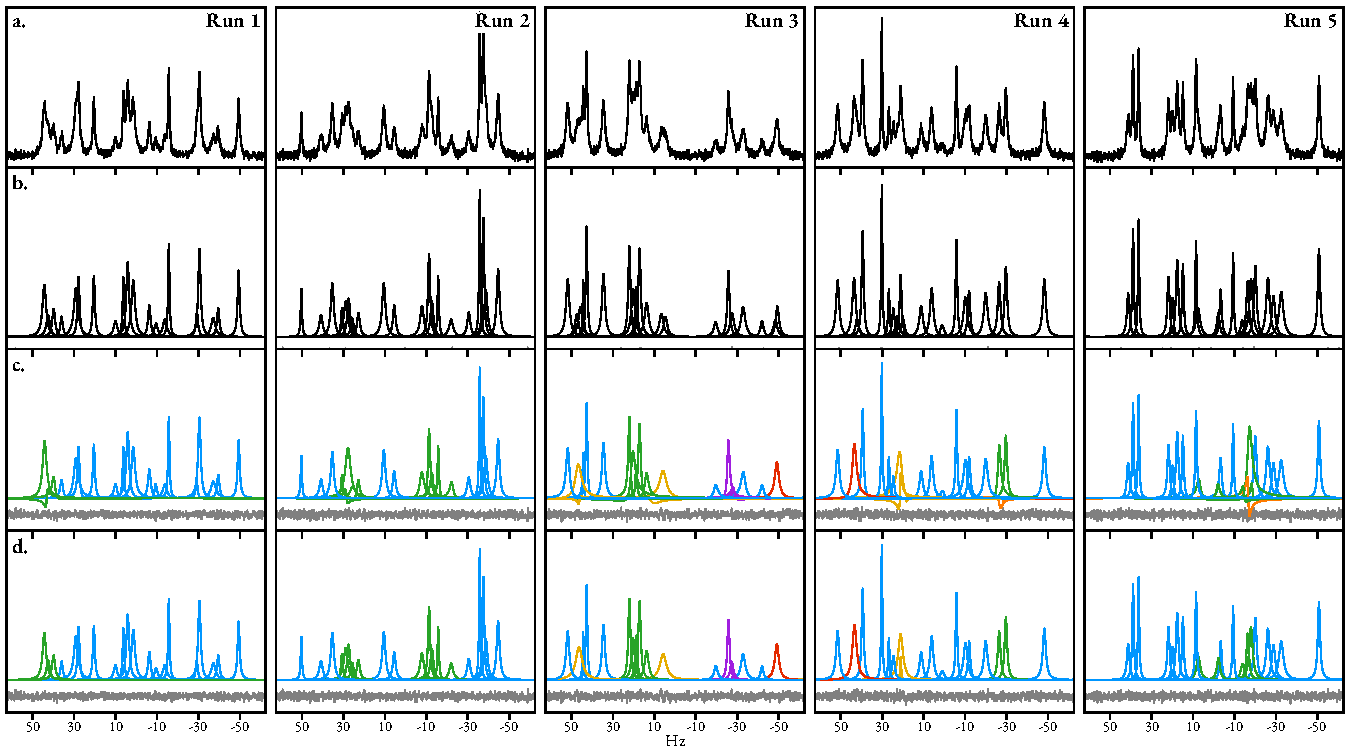
\includegraphics{mpm_vs_nlp/mpm_vs_nlp.pdf}
    \caption[
        The result of estimating a series of 5 simulated signals comprising 20
        oscillators, using solely the \acs{MPM} and also with phase
        variance-regularised \acs{NLP} afterwards.
    ]{
        The result of estimating a series of 5 simulated signals comprising 20
        oscillators (see the main text for details on how the datasets were constructed).
        \textbf{a.} Spectra of the datasets generated.
        \textbf{b.} Plots of spectral lines for each oscillator generated using
        the \acs{MPM}.
        \textbf{c.} An equivalent plot for the result after applying \acs{NLP},
        with the \ac{MPM} result being the initial guess.
        \textbf{d.} Spectral lines corresponding to the true set of oscillators
        used to generate each the datasets.
        Also included in \textbf{b.} -- \textbf{d.} is the residual between the
        data and the sum of the oscillator peaks (grey line).
        The colouring of oscillator lines is described in the main text.
    }
    \label{fig:mpm_vs_nlp}
\end{sidewaysfigure}
